% Ch5.tex

\chapter{Multiple-instance multiple-label learning for the classification of frog calls with acoustic event detection}
\label{cha:cha6MIML}


\section{Overview}
\label{sec:intro}

This chapter presents a method for the classification of simultaneously vocalising frog species in low signal-to-noise ratio (SNR) recordings. In Chapters \ref{cha:cha4EnhancedFeature} and \ref{cha:cha5WaveletFeature}, frog call classification is solved using a signal-instance single-label (SISL) framework, which cannot reflect the nature of automatically collected environmental recordings. Most automatically collected field recordings have low SNR and consist of multiple simultaneous animal vocal activities including frogs, birds, crickets, and so on. This character of environmental acoustic recordings makes the multiple-instance multiple-label (MIML) learning a suitable classification framework. To be specific, individual frog syllables in one audio clip are regarded as \textit{multiple instance}, and the frog species included in that audio clip denote \textit{multiple labels}. 
The key part of this MIML classification framework for studying frog calls is to detect individual syllables in environmental recordings with multiple simultaneously vocalising frog species. After syllable detection, standard acoustic features and MIML classifiers can be used to perform the MIML classification.


To evaluate our proposed MIML classification framework, a representative sample of 342 10-second recordings was exported from the database and split into training and testing sets. The performance is evaluated based on the MIML learning measures. Experimental results demonstrate that the MIML classification framework can be successfully adopted to classify multiple simultaneously vocalising frog species in low SNR recordings.



\section{Materials and methods}
Our frog call classification system consists of
four steps: signal processing, acoustic event detection, feature
extraction, and classification (Fig.~\ref{fig:flowchart}). Detailed description of each step is listed in the following sections. 

\begin{figure}[htb!]
\centering
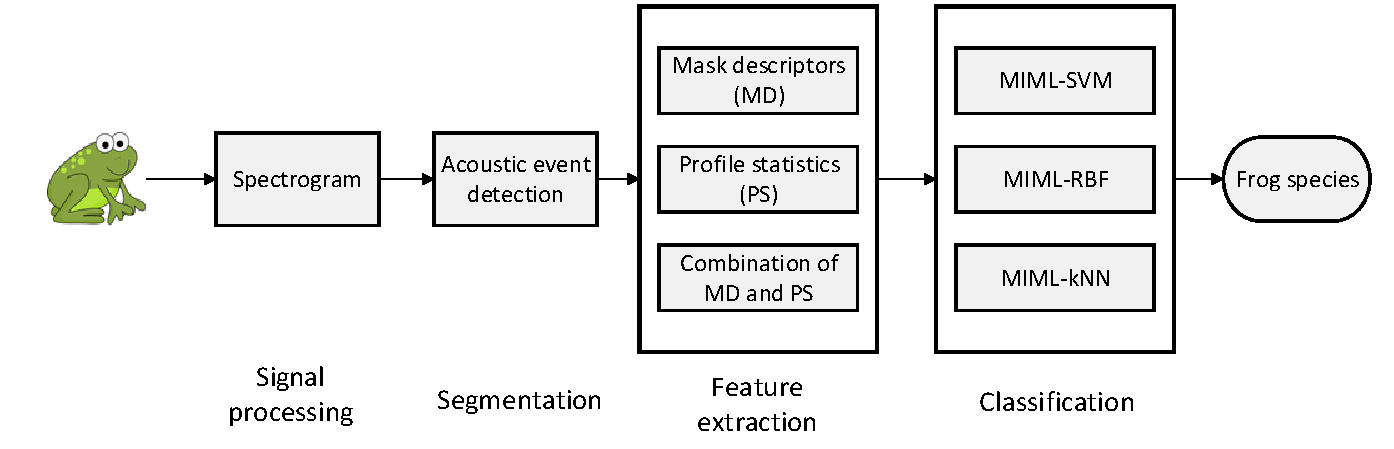
\includegraphics[width=\textwidth]{image/Ch6/flowchart.pdf}
\caption{Flowchart of a frog call classification system using MIML learning}
\label{fig:flowchart}
\end{figure}



\subsection{Materials}
\label{chap5:Materials}
Digital recordings in this chapter were obtained with a battery-powered, weather-proof acoustic sensors. Recordings were two-channel, sampled at 22.05 kHz and saved in WAV format. In this chapter, a representative sample of 342 10-second recordings was selected to train and evaluate our proposed algorithm for predicting which frog species are present in a 10-second recording. All those examples were collected between February 2014 to April 2014, because it is the breeding season for frogs in Queensland, Australia with high calling activities. All the 10-second recordings were manually labelled by an ecologist with eight frog species: Canetoad (CAD) 
($F_{0}$=560 Hz), Cyclorana novaehollandiae (CNE) ($F_{0}$=610 Hz), Limnodynastes terraereginae (LTE) ($F_{0}$=610 Hz), Litoria fallax (LFX) ($F_{0}$=4000 Hz), Litoria nasuta (LNA) ($F_{0}$=2800 Hz), Litoria rothii (LRI) ($F_{0}$=1800 Hz), Litoria rubella (LRA) ($F_{0}$=2300 Hz), and Uperolela mimula (UMA) ($F_{0}$=2400 Hz). Here, $F_{0}$ is the averaged dominant frequency for each frog species. Each recording includes between 1 and 5 species. Following the prior work of \cite{briggs2012acoustic}, we assume that recordings without  frog vocalisations can be filtered out during the acoustic event detection process.


\subsection{Signal processing}
All the recordings were first re-sampled at 16 kHz and mixed to mono. A spectrogram was then generated by applying short-time Fourier transform (STFT) to each recording. Specifically, each recording was
divided into frames of 512 samples with 50\% frame overlap.
A fast Fourier transform was then performed on each frame with a Hamming window, which yielded amplitude values for 256 frequency bins, each spanning 31.25 Hz. The final
decibel values (S) were generated as 
\begin{equation}
S_{tf} = 20*log_{10}(A_{tf})
\end{equation}
where $A$ denotes the amplitude value, $t=0,...,T-1$ and $f=0,...,F-1$ represent time and frequency index, $T$ and $F$ are 256 frequency bins and 625 frames, respectively. 

\subsection{Acoustic event detection for syllable segmentation}
The aim of acoustic event detection (AED) is to detect a specified acoustic event in audio data. In this chapter, we use AED for frog syllable segmentation. Since all the recordings are collected from the field, there are many overlapping vocal activities from different sources. Traditional methods for frog syllable segmentation are based on time domain information \cite{somervuo2004classification,huang2009frog}, which cannot address those recordings. Here, we modified the AED method developed by Towsey et al. \cite{towsey2012toolbox} for syllable segmentation. The detail of our AED method is described as follows:
\\
\textbf{Step 1:} Wiener filtering 

\noindent A 2-dimensional Wiener filter is applied to the spectrogram image over a $5 \times 5$ time-frequency grid for reduce the background graininess, where the filter size is selected after the consideration of trade-off between removing the background graininess and blurring the acoustic events.
\begin{equation}
\hat{S_{tf}} = \mu + \frac{(\sigma^{2}-\nu^{2})}{\sigma^{2}}(S_{tf}-\nu)
\end{equation}
where $\mu$ and $\sigma^{2}$ are local mean and variance, respectively; $\nu^{2}$ is the noise variance estimated by averaging all local variances. 
\\
\textbf{Step 2:} Spectral subtraction

\noindent Wiener filtering can successfully remove the graininess, but some noises, such as wind,
insect, motor engine that cover the whole recording can not be addressed using Wiener filtering. Here, a modified spectral subtraction method is employed to deal with those noises. 


\begin{algorithm}
\DontPrintSemicolon
\KwData{$\hat{S_{tf}}$, spectrogram after Wiener filtering.}
\KwResult{$\hat{S^{'}_{tf}}=\hat{S_{tf}}$, noise reduced spectrogram.}

\Begin{
%$V \longleftarrow U$\;
%$S \longleftarrow \emptyset$\;
\textbf{Construct} an array of the modal noise values for all frequency bins;

\For{$f\in F$}{
\textbf{1}. calculate the histogram of the intensity value over each frequency bin 

\textbf{2}. smooth the histogram array with a moving average window of size 7

\textbf{3}. regard the modal noise intensity at the position of maximal bin in the left-side of the histogram
}


\textbf{Smooth} the array with a moving average filter with window of size 5;

\For{$f\in F$}{
\textbf{1}. subtract the modal noise intensity

\textbf{2}. truncated negative decibel values to zero
}
}  
\caption{Modified Spectral Subtraction\label{IR}}

\end{algorithm}

\noindent \textbf{Step 3:} Adaptive thresholding

\noindent After noise reduction, the next step is to convert a noise reduced spectrogram $\hat{S^{'}_{tf}}$ into the binary spectrogram $S^{b}_{tf}$ for the event detection. Here, an adaptive thresholding method named \textit{Otsu thresholding} \cite{otsu1975threshold} is employed to find an optimal threshold.

\begin{equation}
\phi_{b}^{2}(k)=w_{1}(k)w_{2}(k)[\mu_{1}(k)-\mu_{2}(k)]^{2}
\end{equation}
\noindent where $w_{1}(k)=\sum_{0}^{k}p(j)$ is calculated from the histogram as $k$, $p(j)=n(j)/N$ are the values of the normalised gray level histogram, $n(j)$ is the number of values in level $j$, $N$ is the total number of values over the whole spectrogram image, $\mu_{1}(k)=[\sum_{0}^{k}p(j)x(j)]/w_{1}$, $x(j)$ is the value at the center of the $j$th histogram bin. Then, the threshold, $T_{0}$, is calculated as

\begin{equation}
T_{0}= (\phi_{b1}^{2}(k) + \phi_{b2}^{2}(k)) / 2
\end{equation}

\noindent \textbf{Step 4:} Events filtering using dominant frequency and event area \\
Since not all detected events correspond to frog vocalisations, to further remove those events that are not from the listed frog species in section \ref{chap5:Materials}, dominant frequency ($F_{0}$) and area of the event ($Ar$) are used for filtering.


\begin{algorithm}
\DontPrintSemicolon
\KwData{ $S^{b}_{tf}$, spectrogram; $t_{s}(n)$, $t_{e}(n)$, $f_{l}(n)$, $f_{h}(n)$, location of each acoustic event $n$; $F_{0}(i)$, dominant frequency of frog species $i$.}
\KwResult{ $\tilde{S_{tf}}$, spectrogram after events filtering.}

\Begin{
%\textbf{Step 1:} separate large acoustic events
%\\
\textbf{Calculate} the area of each acoustic event $n$.
$Area(n)=(t_{e}(n)-t_{s}(n))*(f_{h}(n)-f_{l}(n))$

\For{$n \in N_{e1}$}{
\If{$Ar(n) \geq Ar_{l}$}{
split event $n$ into small events
}
} 
where $Ar_{l}$ is set as 3000 pixels.\\
%\textbf{Step 2:} dominant frequency 
\textbf{Filter} events using dominant frequency
$f_{d}(n)= \sum_{t=t_{s}(n)}^{t_{e}(n)} F(t) / t_{e}(n)-t_{s}(n)$ \\
where $F(t)$ is the peak frequency of each frame within the event area


\For{$n \in N_{e2}$}{
\For{$i \in I$}{
\If{$f_{d}(n) \geq F_{0}(i)+\theta$; $f_{d}(n) \leq F_{0}(i)-\theta$}{
	$f_{d}(n) =0$;
}
}}
where $\theta$ is frequency range and set as 300 Hz.

\textbf{Remove} small acoustic events except frequency band between $\theta_{l}$ and $\theta_{h}$
\\
\For{$n \in N_{e2}$}{
\If{$Ar(n) \leq Ar_{s}$}{
remove event $n$
}
} 
where $Ar_{s}$ is set as 300 pixels, $\theta_{l}$ and $\theta_{h}$ are set as 300 Hz and 800 Hz, respectively. Because the area of LTE is smaller than $Ar_{s}$.
}
\caption{Event filtering based on dominant frequency and event area}
\end{algorithm}




\noindent \textbf{Step 5:} Region growing
\\
A region growing algorithm is used to obtain the contour of the particular acoustic event \cite{mallawaarachchi2008spectrogram}. To get the accurate boundary of each acoustic event and improve the discrimination of extracted features, a 2-dimensional region growing algorithm is applied to obtain the accurate event shape within each segmented event. First, a maximal intensity value within the event area is selected as the seed point. Then, the neighbourhood pixels of the seed(s) above the threshold are located and assigned to the output image, and new added pixels are used as seeds for further processing. Finally, when all the pixels that satisfy the criteria are added to the output image, the recursive algorithm will stop and get the final results (Figure~\ref{fig:Ch6_AED}). Here, the threshold value is empirically set as 5 dB.

\begin{figure}[htb!]
\centering

        \begin{subfigure}[b]{0.45\textwidth}
                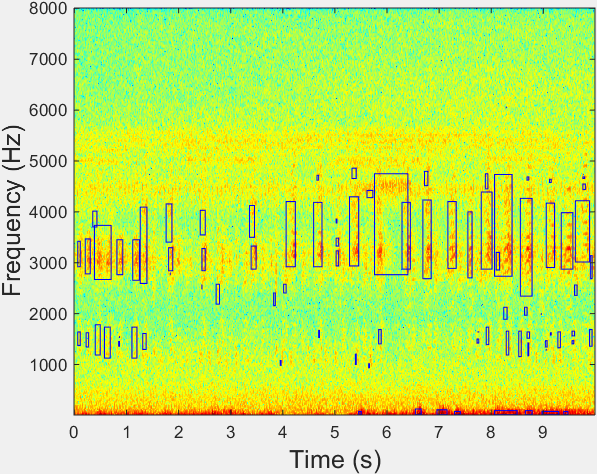
\includegraphics[width=\textwidth]{image/Ch6/AEoriginal.png}
                %\caption{ }
        \end{subfigure}
       ~
              \begin{subfigure}[b]{0.45\textwidth}
                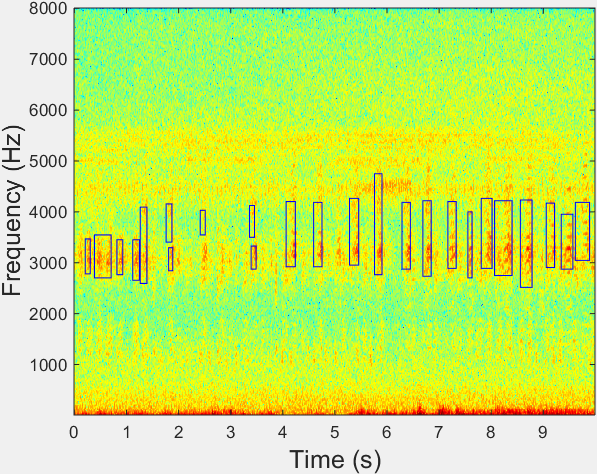
\includegraphics[width=\textwidth]{image/Ch6/AEfinal.png}
                
        \end{subfigure}  
     
\caption[Acoustic event detection results before (Left) and after (Right) event filtering based on dominant frequency]{Acoustic event detection results before (Left) and after (Right) event filtering based on dominant frequency. Here, blue rectangle means the time and frequency boundary of each detected event.}
        \label{fig:feature}
\end{figure}

\begin{figure}[htb!]
\centering
        \begin{subfigure}[b]{0.45\textwidth}
                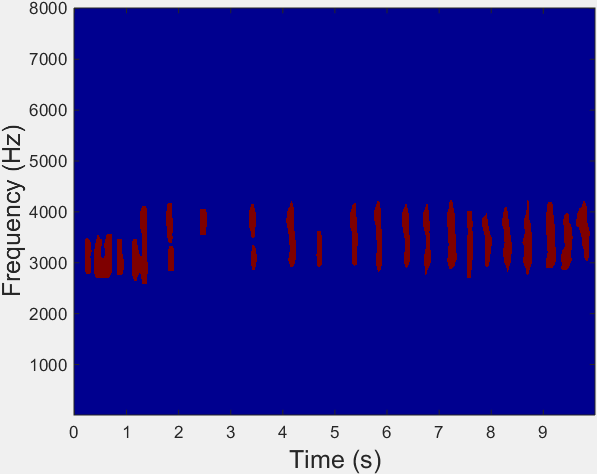
\includegraphics[width=\textwidth]{image/Ch6/binary.png}
                %\caption{ }
        \end{subfigure}
       ~
              \begin{subfigure}[b]{0.45\textwidth}
                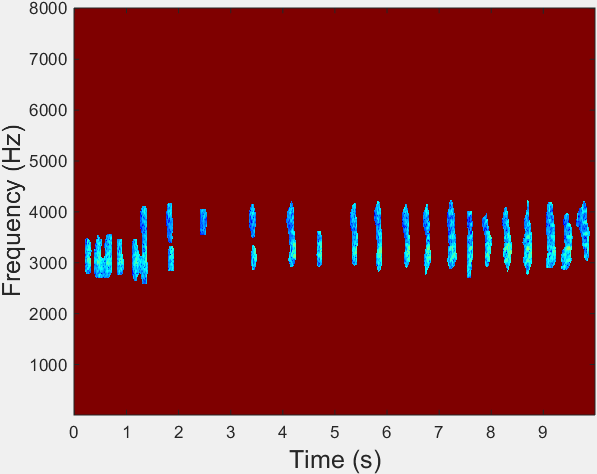
\includegraphics[width=\textwidth]{image/Ch6/segmentEvents.png}                
        \end{subfigure}       
\caption[Acoustic event detection results after region growing]{Acoustic event detection results after region growing. Left: binary segmentation results; Right: segmented frog syllables.}
        \label{fig:Ch6_AED}
\end{figure}



\subsection{Feature extraction}
Based on acoustic event detection results, two feature representations are first calculated to describe each event (syllable): mask descriptors and profile statistics \cite{briggs2012acoustic}. Here, we exclude \textit{histogram of orientation (HOG)} from our feature set, because the previous studies have already demonstrated its lowest classification accuracy \cite{briggs2012acoustic, ruizmultiple2015}. For mask descriptors, it is used to describe the syllable shape including minimum frequency, maximum frequency, bandwidth, duration, area, perimeter, non-compactness, rectangularity. For profile statistics, there are time-Gini, frequency-Gini, frequency-mean, frequency-variance, frequency-skewness, frequency-kurtosis, frequency-max, time-max, mask-mean, and mask standard deviation. The third feature set consists of all features.







\subsection{Multiple-instance multiple-label classifiers}
After feature extraction, three MIML algorithms are evaluated for the classification of multiple simultaneous vocalising frog species: MIML-SVM, MIML-RBF, and MIML-kNN. With the form of event-level distance measure, the MIML problem can be reduced to a single-instance multiple-label problem by associating each event with an event-level feature \cite{briggs2012acoustic}. Here, the maximal and average Hausdorff distances between two syllables are used by MIML-SVM and MIML-RBF, separately. For MIML-kNN, the nearest neighbour is used to assign syllable-level features. 


\section{Experiment results}

\subsection{Parameter tuning}
There are three modules, the parameters of which need to be discussed: signal processing, acoustic event detection, and classification. For signal processing, the window size and overlap are 512 samples and 50\%, respectively. During the process of acoustic event detection, four thresholds for event filtering need to be determined, which are small and large area threshold, and frequency boundary for events filtering. All those thresholds were determined empirically by applying various combinations of thresholds to a small number of randomly selected 10-second clips. For MIML-SVM classifiers, the parameters used are ($C,\gamma,r$) and set as (0.1, 0.6, 0.2) experimentally. For MIML-RBF, the parameters are ($ r, \mu$) and set as (0.1,0.6). For MIML-kNN, the number of references (k) and citers ($k^{'}$) are 10 and 20, respectively.
 
%Five measures including Hamming loss, rank loss, one-error, coverage, and micro-AUC are used to characterize the accuracy of each algorithm \cite{zhou2008miml, dimou2009empirical}. The definition of each measure can be found in \cite{briggs2012acoustic}
\subsection{Classification}
In this chapter, all the algorithms were programmed in Matlab 2014b. Each MIML algorithm is evaluated with five-fold cross-validation on the collection of 342 species-labelled recordings. 
Five evaluation rules are used for comparing the performance with the combination of three feature representations and three ML algorithms: Hamming loss, Rank loss, Average precision, One error, Exampled based F1, and Micro F1 \citep{Madjarov20123084, zhou2008miml}. The value range of all five evaluation rules is between 0 to 1. The definition of each evaluation rule is described as follows:
\\
\textbf{1)} Hamming loss is defined as the fraction of labels that are incorrectly predicted for an instance and the normalised Hamming loss which is normalised over instances is reported. This metric is defined as
\begin{equation}
hammingLoss = \frac{1}{N}\sum_{i=1}^{N}\frac{1}{Q}|h(x_{i})\Delta y_{i})|
\end{equation}
where $\Delta$ denotes the symmetric difference between two instances, $N$ is the number of instances and $Q$ is the total number of possible labels. $y_{i}$ denotes the ground truth of instance $x_{i}$, and $h(x_{i})$ denotes the predictions for the same instance. 
\\
\textbf{2)} Ranking loss evaluates the average fraction of label pairs that are reversely ordered for the particular instance given by
\begin{equation}
rankingLoss = \frac{1}{N}\sum_{i=1}^{N}\frac{|D_{i}|}{|y_{i}||\bar{y_{i}}|}
\end{equation}
where $D_{i}={(\lambda_{m},\lambda_{n})| f(x_{i}, \lambda_{m}) \leq f(x_{i}, \lambda_{n}), (\lambda_{m}, \lambda_{n}) \in y_{i} \times \hat{y_{i}}}$,
while $\bar{y}$ denotes the complementary set of $y$ in $L$, and $L={\lambda_{1}, \lambda_{2}, \lambda_{3},..., \lambda_{Q}}$, $\lambda$ represents the label.
\\
\textbf{3)} Average precision is the average fraction of labels that are ranked higher than an actual label belonging to an instance. 
\begin{equation}
precision = \frac{1}{N}\sum_{i=1}^{N}\frac{h(x_{i}) \cap y_{i}}{|y_{i}|}
\end{equation}
\\
\textbf{4)} One error evaluates how many times the top-ranked label is
not in the set of relevant labels of the instance. This evaluation metric is defined as

\begin{equation}
oneError = \frac{1}{N}\sum_{i=1}^{N}[[argmax_{\lambda \in y} f(x_{i},\lambda)] \not \in y_{i} ]
\end{equation}
\\
\textbf{5)}
Exampled based $F_{1}$ is the average of the harmonic mean of instance-precision and instance-recall for every instance. The instance-precision is defined for an instance as the size of the intersection of the set of its predicted labels and the set of its ground truth labels divided by the size of the set of its predicted labels. The instance-recall is defined for an instance as the size of the intersection of the set of its predicted labels and the set of its ground truth labels divided by the size of the set of its ground truth labels.
\begin{equation}
macroF_{1}=\frac{1}{Q}\sum_{j=1}^{Q}\frac{2 \times p_{j} \times r_{j}}{p_{j}+r_{j}}
\end{equation}
where $p_{j}$ and $r_{j}$ are the precision and recall for all $\lambda_{h} \in h(x_{i})$ from $\lambda_{j} \in y_{j}$.
\\
\textbf{6)}
Micro $F_{1}$ is the harmonic mean of micro-precision and micro-recall, where micro-precision and micro-recall are the precision and the recall which are averaged over all instances and label pairs. 
\begin{equation}
microF_{1} = \frac{2 \times microPrecision \times microRecall}{microPrecision + microRecall}
\end{equation}

The values for Hamming loss, rank loss, one-error, coverage, and micro-AUC range from 0 to 1. For Hamming loss, Rank loss, one-error and coverage, 0 denotes the perfect result, and 1 means the wrong prediction of all labels over every instance, whereas for micro-AUD, the values
have the completely opposite meanings. 

The $\frac{positive}{negative}$ is defined as $1-hammingLoss$ and it is 0.818 for MIML-RBF with Mask descriptors (MD). MD and profile statistical (PS), and all features (AF) are put into the three classifiers, respectively. The accuracy measure for each MIML classifier is shown in Table \ref{tab:accuracy}. Here, the best classification accuracy is achieved using MIML-RBF with MD. For each classifier, the classification accuracy of MD is higher than PS and AF, which indicates that the event shape has a better discriminability than the event content. To give a concrete view of predictions, the results of five randomly selected recordings using MIML-RBF are shown in Table~\ref{tab:prediction}. From the table, we can see that recordings of No.1 and No.3 are accurately predicted. 




\begin{table}[htb!]
\centering
\caption[Accuracy measure for MIML classifiers with different feature representations]{Accuracy measures for MIML classifiers with different feature representations. Here, $\downarrow$ indicates ‘the smaller the better’, while ‘$\uparrow$’ indicates ‘the bigger the better’.}
\label{tab:accuracy}
\resizebox{\textwidth}{!}{
\begin{tabular}{lllllll}
\hline\hline
{\bf Feature} & {\bf Algorithm} & {\bf Hamming loss $\downarrow$} & {\bf Rank loss $\downarrow$} & {\bf One-error $\downarrow$} & {\bf Coverage $\downarrow$} & {\bf Micro-AUC $\uparrow$} \\ \hline
MD            & MIML-SVM        & 0.253              & 0.186           & 0.308           & 3.147          & 0.745           \\ 
MD            & MIML-kNN        & 0.205              & 0.153           & 0.298           & 2.647          & 0.771           \\ 
MD            & MIML-RBF        & {\bf 0.182}        & {\bf 0.132}     & {\bf 0.223}     & {\bf 2.352}    & {\bf 0.828}     \\ 
PS            & MIML-SVM        & 0.239              & 0.208           & 0.323           & 3.544          & 0.728           \\ 
PS            & MIML-kNN        & 0.211              & 0.153           & 0.298           & 2.647          & 0.777           \\ 
PS            & MIML-RBF        & 0.186              & 0.161           & 0.338           & 3.161          & 0.746           \\ 
AF (MD+PS)            & MIML-SVM        & 0.261              & 0.199           & 0.279           & 3.588          & 0.761           \\ 
AF (MD+PS)               & MIML-kNN        & 0.205              & 0.160           & 0.264           & 2.735          & 0.787           \\ 
AF (MD+PS)              & MIML-RBF        & 0.191              & 0.142           & 0.220           & 2.632          & 0.821           \\ \hline\hline
\end{tabular}
}
\end{table}



\begin{table}[htb!]
\centering
\caption{Example predictions with MIML-RBF.}
\label{tab:prediction}
\begin{tabular}{lll}
\hline\hline
{\bf No.} &{\bf Ground truth} & {\bf Predicted labels} \\ \hline
1&UMA                & UMA                    \\ 
2&LNA, LRI, UMA      & LNA, LRA, UMA          \\ 
3&LNA, UMA           & LNA, UMA               \\ 
4&LNA, LFX, LRA      & LNA, LFX, LRI, LRA     \\ 
5&LNA, LFX, LRA      & LNA, LRA               \\ \hline\hline
\end{tabular}
\end{table}



\section{Discussion}
Since most recordings used in this chapter consist of multiple simultaneously vocalising frog species, the traditional single-instance single-label classification framework is no longer suitable. A novel framework for the classification of multiple simultaneous vocalising frog species in environmental recordings is proposed, which is adopted from \cite{briggs2012acoustic}, a study on birds. Differently from that work, this research designs a new acoustic event detection method for syllable segmentation rather than using a supervised learning algorithm. It is because there is a lack of lots of annotated frog recordings. As for the classification results, our proposed framework can achieve an acceptable classification accuracy. All the features used in this study are calculated from the segmented syllables. The accuracy of the segmentation results will therefore directly affects the final classification performance.


\section{Summary and limitations}
In this chapter, we propose a novel framework for the classification of multiple simultaneous vocalising frog species in environmental recordings. To the best of our knowledge, this is the first study that focuses on the frog recordings using the MIML algorithm. Since frogs tend to call simultaneously, the MIML algorithm is more suitable for dealing with those recordings than single-instance single-label classification. After applying an acoustic event detection algorithm to 10-second recordings, frog syllables are segmented. Then, three feature representations, MD, PS, and AF, are calculated from those segmented syllables. Finally, three MIML classifiers are used for the classification of frog calls with the best true positive/negatives of 81.8\%. Future work will focus on the study of novel features and MIML classifiers to further improve the classification performance. Current classification results are highly affected by the syllable segmentation results, and the use of AED can not accurately segment all the syllables. One solution is to prepare an annotated dataset and apply supervised learning algorithms for the segmentation task. Another is to use a different classification framework, which does not need the segmentation process.  


